%!TEX root = ../../../adrien_gomar_phd.tex

\section{Introduction}
\label{sec:ca_introduction}

In the seventies, the two oil crisis showed the aeronautical industries its dependence
toward energy resources. To face this issue, the U.S. Senate directed NASA in $1975$
to look for every potential fuel-saving concept. The Advanced Turboprop
project was born~\cite{Hager1988}. The reflection led to the
concept of contra-rotating open rotor.

In an airplane engine, 
the thrust $F_x$ and the propulsive efficiency $\eta_{pr}$ are given by:
\begin{equation}
  \begin{split}
    F_x &= Q \Delta V, \\
    \eta_{pr} &= \displaystyle \frac{1}{1 + \displaystyle \frac{\Delta V}{2 V_0}},
  \end{split}
\end{equation}
where $Q$ is the mass-flow, $\Delta V$ is the inlet/outlet velocity difference and $V_0$
the inlet velocity. These equations means that the 
smaller the velocity difference $\Delta V$, the higher the propulsive efficiency.
Then, to increase the thrust $F_x$ which is the reason being of an engine,
the only way is to work on the mass-flow $Q$.
The current

In this way, a propeller is more efficient than a jet. In fact, a jet 
moves small mass of gas at high velocity while propellers moves 
large mass of air at low velocity, increasing the propulsive efficiency.

Only ten years later, the cost of 
the barrel decreased for twenty years to almost retrieve its original
value. 

In the beginning of the eighties, the cost of 
the barrel decreased for almost twenty years and then increased again.
Today, the cost of a barrel is almost at its maximum as shown
in Fig.~\ref{fig:crude_oil_price}.
\begin{figure}[htbp]
  \centering
  \includegraphics*[width=0.40\textwidth]{crude_oil_price.pdf}
  \caption{Evolution of the cost of a barel from $1861$ to $2012$ \cite{bpreview2013}}
  \label{fig:crude_oil_price}
\end{figure}

Nevertheless, Airbus forecast a doubled number of passengers in
$2031$. To allow a sustainable air transportation, the aeronautical
industry should reduce its environmental footprint. For instance,
the European Commission recently published the \emph{Flightpath $2050$}.
In this document, the aeronautical industries are set goals for $2050$
shown in Fig.~\ref{fig:flightpath_2050}.
\begin{figure}[htbp]
  \centering
  \includegraphics*[width=0.40\textwidth]{flightpath_2050.pdf}
  \caption{European Commission goals for the aeronautical industry. }
  \label{fig:flightpath_2050}
\end{figure}
The noise, CO2 and NOx emissions should be reduced of 
respectively $65\%$, $75\%$ and $80\%$.
These are ambitious goals, needing technological breakthrough.

The main source of pollutant emission is the engine. Two ways of reducing
these are through a better control of the combustion and better
efficiency of the device in global.

How to increase the mass-flow ??
HBR or propeller

The basic idea behind the CROR concept is that a propeller has a 
better propulsive efficiency than a turbofan. The problem is that
a residual tangential velocity is present behind a propeller.
In fact, applying the velocity triangle to a propeller configuration
as shown in Fig.~\ref{fig:ca_velocity_triangle_propeller}, one can
observe that the outlet velocity (noted $V^{out}_x$) is not axial
leading a tangential velocity $\Delta V_{\theta}$. This tangential forms
the swirl observe behind a propeller. First, this is a lost energy and
second, it produces a torque that has an impact on the flight dynamics
of the aircraft. To alleviate this effect, one can use two propellers
that are counter-rotating as for instance the TP$400$ propellers
in the Airbus-A$400$M military airplane.

To recover this lost energy, a second contra-rotating rotor is used.
\begin{figure}[htb]
  \centering
  \subfigure[propeller]{
    \label{fig:ca_velocity_triangle_propeller}
    \includegraphics*[scale=0.4]{velocity_triangle_propeller.pdf}}
  \subfigure[contra-rotating open rotor]{
    \label{fig:ca_velocity_triangle_cror}
    \includegraphics*[scale=0.4]{velocity_triangle_cror.pdf}}
  \caption{Velocity triangle applied to a propeller and a 
  contra-rotating open rotor configuration.}
\end{figure}
Figure~\ref{fig:ca_velocity_triangle_cror} shows the application
of the velocity triangle to a CROR configuration. The swirl
energy that was lost in the propeller is now used to 
produce more thrust. Thus, a CROR has a better propulsive
efficiency than a propeller.

The contra-rotating open rotor architecture is a classical engine
turbomachinery whose fan is not within a nacelle. As explain
above, this help increasing the mass-flow of the primary flow
which leads to a higher propulsive efficiency.
Two main architectures are retained. One based on a gearbox, the second
being build around a statorless low-pressure turbine.
\begin{figure}[htb]
  \centering
  \subfigure[Geared design]{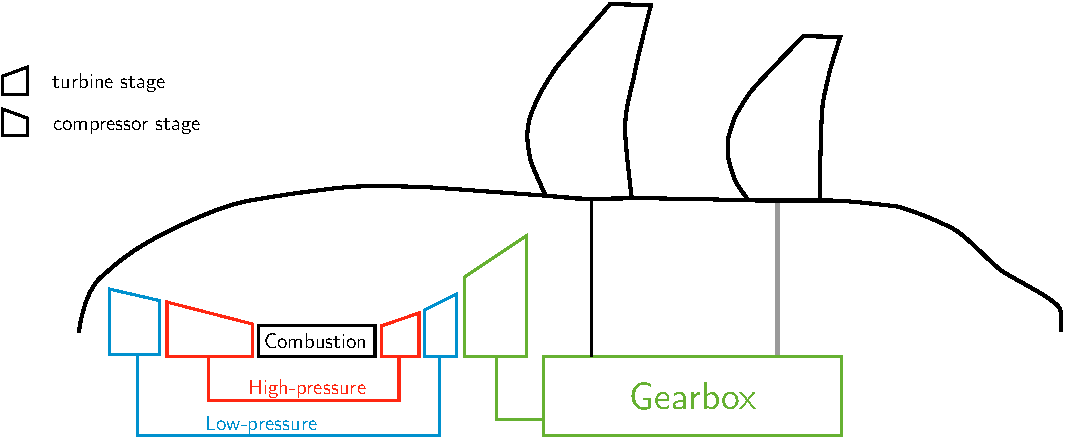
\includegraphics[width=.4\textwidth]{geared_cror.pdf}}
  \subfigure[Statorless low-pressure turbine design]{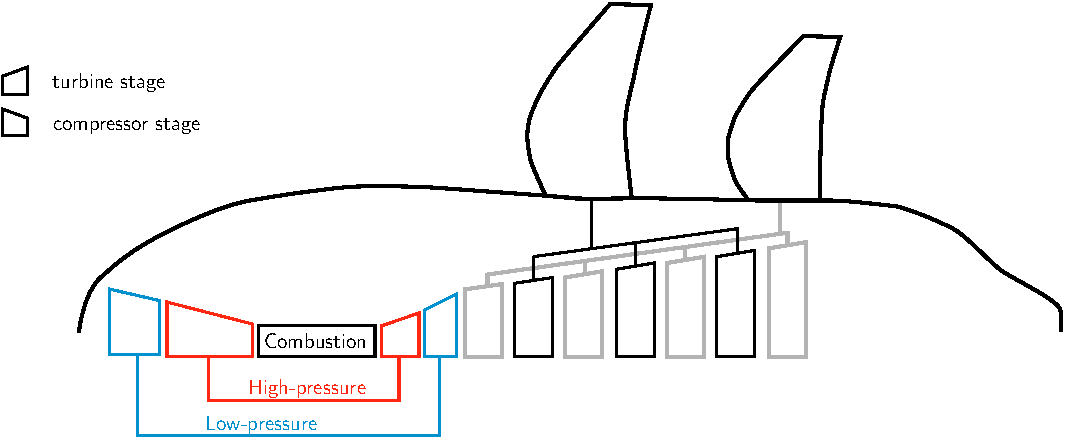
\includegraphics[width=.4\textwidth]{stator_less_cror.pdf}}
  \caption{Contra-rotating open rotor architectures.}
  \label{fig:ca_cror_designs}
\end{figure}



\section{Geometry}
\label{sec:ca_geometry}

Figure~\ref{fig:ca_cror_geometry} depicts the main
geometrical parameters of a CROR.
It is composed of two rotors, the first one is called
the front rotor and the second one is called the rear or aft rotor.
The two rotors do not have the same diameter $D$ and rotation speed
$\Omega$. Thus, subscript $F$ and $R$ denotes respectively,
the front and the rear parameter. The diameter is expressed in meters
while the rotation speed is expressed in radians per seconds.
As the rotors are contra-rotating, their rotation speed is opposed.
The absolute value of the rotation speed is not necessarily the same,
as it depends on the chosen architecture. Therefore not assumption
will be made on the relation between the front and the rear
rotation speed.
The difference of diameters is called the clipping or cropping
of the blades and is evaluated as through the non-dimensional parameter
$\kappa$:
\begin{equation}
    \kappa = \frac{D_F - D_R}{D_F}.
\end{equation}
This is done to avoid the interaction of the tip vortex generated
by the front rotor with the rear rotor.
Finally, the spacing between the rotors
is evaluated as the difference between the axial minimum of the
rear blade minus the maximum of the front blade. This parameter
helps reducing the noise produced by the interaction of
the rotors through the potential effects.
\begin{figure}[htbp]
  \centering
  \includegraphics*[width=0.40\textwidth]{cror_geometry.pdf}
  \caption{Contra-rotating open rotor geometrical parameters.}
  \label{fig:ca_cror_geometry}
\end{figure}

\section{Integrated parameters: the similarity coefficients}
\label{sec:ca_similarity_coeff}

To allow the comparison and the assessment of several
CROR configurations, four similarity coefficients are used:
the advance ratio $J$, the traction coefficient $C_t$, 
the power coefficient $C_p$ and the efficiency $\eta$.
These are defined for a rotor as:
\begin{equation}
    J = \frac{V_0}{n D}, \quad
    C_t = \frac{F_x}{\frac{1}{2} n ^ 2  D ^ 4}, \quad
    C_p = \frac{M_x \Omega}{\frac{1}{2} n ^ 3 D ^ 5}, \quad
    \eta = J \frac{C_t}{C_p},
\end{equation}
where $V_0$ is the free-stream velocity (depicted in Fig.~\ref{sub:ca_geometry}), 
$n$ the rotation frequency ($n = \Omega / 2 \pi$), 
$F_x$ and $M_x$, respectively, the axial force torque.

In the case of a CROR configuration, two rotors are considered.
Two main ways exists to evaluate the global value of the
similarity coefficients. The first one, chosen by
\citet{Bechet2011} among others, is to consider
that the non-dimensioning parameter $D$, $n$ and $J$ are those
of the front rotor for both rotors. 
The second one uses the non-dimensioning parameter of the current rotor,
as done by \citet{Stuermer2008} and \citet{Zachariadis2011}.
The traction and power coefficients of the rear rotor is
computed using its own advance ratio, diameter and rotation frequency.
Nevertheless, computing the advance ratio of the rear rotor, as
the freestream velocity should be updated to take into account
for the acceleration generated by the front rotor. The freestream
velocity is chosen to be $V_0$, which is of course not true.
The efficiency is computed rotor per rotor and then
assembled through an arithmetic addition. This is the approach retained
in this thesis.

An estimation of the variation of the advance ratio $J$ and the 
efficiency $\eta$ depending on the flight conditions can be given as follow
\begin{alignat}{4}
    \text{(cruise)} \quad  0.8 &< \eta &< 0.95, \quad 1 &< J < 3.5 \\
    \text{(take-off)} \quad  0.5 &< \eta &< 0.8, \quad J &< 1.
\end{alignat}

\section{Three-dimensional flow}
\label{sec:ca_3D_flow}



\section{The mean stationary flow}
\label{sec:ca_general_flow_physics}

Now that the average values of the integrated parameters are given,
one can focus on more local information. Here, we will first use
the azimuthal average variations. These are computed by extracting
an axial plane and azimuthally averaging the field. If $f(x, r, \theta)$
denotes the evolution of the field then its azimuthal variation at
an axial position $x_0$ is:
\begin{equation}
    f(x=x_0, r) = \int_{\theta} f(x=x_0, r, \theta) \diff \theta.
\end{equation}


% \subsection{General flow physics}
% \label{sub:ca_general_flow_physics}

% In this section, the general flow physic of a CROR configuration
% is detailed for four 

% The range of CROR engines is limited to a subsonic Mach number.
% In fact, the absence of a nacelle implies that the CROR
% will work under the airplane flight conditions. This is
% not the case of a turbofan whose nacelle helps controlling
% the Mach number seen by the fan. Thus the CROR range of operating
% condition is limited to a Mach number $M \leq 0.8$.
